\color{black}
\subsection{Matriz DOFA}
Estas siglas provienen del acrónimo en inglés SWOT (strenghts, weaknesses, opportunities, threats); en español, aluden a fortalezas, oportunidades, debilidades y amenazas. El análisis FODA consiste en realizar una evaluación de los factores fuertes y débiles que, en su conjunto, diagnostican la situación interna de una organización, así como su evaluación externa, es decir, las oportunidades y amenazas. También es una herramienta que puede considerarse sencilla y que permite obtener una perspectiva general de la situación estratégica de una organización determinada. Thompson y Strikland (1998) establecen que el análisis FODA estima el efecto que una estrategia tiene para lograr un equilibrio o ajuste entre la capacidad interna de la organización y su situación externa, esto es, las oportunidades y amenazas. \cite{Dofa}

En la siguiente figura se ilustran los elementos que componen el análisis FODA y como identificarlos:

\vspace{2mm}
\begin{minipage}{0.9\textwidth}
\centering
\captionof{figure}[{Aspectos Matriz DOFA.}]{ Aspectos Matriz DOFA }
\label{dofa}
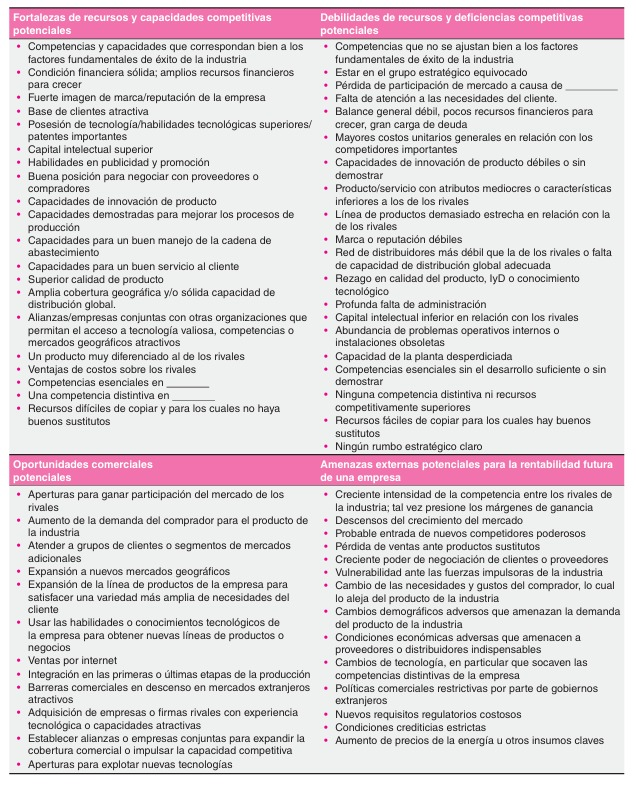
\includegraphics[width=0.6\textwidth]{Content/Images/dofa-ejemplo.jpeg}
\footnote{Nota. \textup{Fuente :Administracion estrategica
\cite{administracion-estrategica}}}
\end{minipage}

Agrupando los elementos del análisis FODA, se pueden identificar cuatro tipos de estrategias:
\begin{itemize}
     \item \textbf{FO(Fortalezas-Oportunidades):}Estas estrategias permiten a la organización crecer y desarrollarse aprovechando al máximo sus capacidades internas y las oportunidades que ofrece el entorno. Por ejemplo, una empresa con una sólida reputación y recursos tecnológicos avanzados puede expandirse a nuevos mercados emergentes o lanzar productos innovadores, capitalizando tanto sus fortalezas como las oportunidades detectadas.
    \item \textbf{DO (Debilidades-Oportunidades):} Estrategias que buscan mejorar las debilidades internas aprovechando las oportunidades externas disponibles. Estas estrategias pueden implicar la inversión en capacitación del personal, la mejora de procesos internos o la adopción de nuevas tecnologías para optimizar el rendimiento y la competitividad de la organización.
    \item \textbf{FA (Fortalezas-Amenazas):} Estrategias que utilizan las fortalezas internas para enfrentar y mitigar las amenazas externas que enfrenta la organización. Por ejemplo, una empresa con una sólida red de distribución puede utilizarla para contrarrestar la competencia agresiva o adaptarse a cambios en las regulaciones del mercado, asegurando así su posición en el sector.
    \item \textbf{DA (Debilidades-Amenazas):} Estrategias defensivas que buscan minimizar las debilidades internas y evitar o reducir el impacto de las amenazas externas en la organización. Estas estrategias pueden incluir la reestructuración de procesos, la mejora de la eficiencia operativa o la diversificación de productos y servicios para reducir la dependencia de un mercado específico.
\end{itemize}

\begin{minipage}{0.9\textwidth}
\centering
\captionof{table}[{ Matriz DOFA.}]{  Matriz DOFA }
\label{dofa}
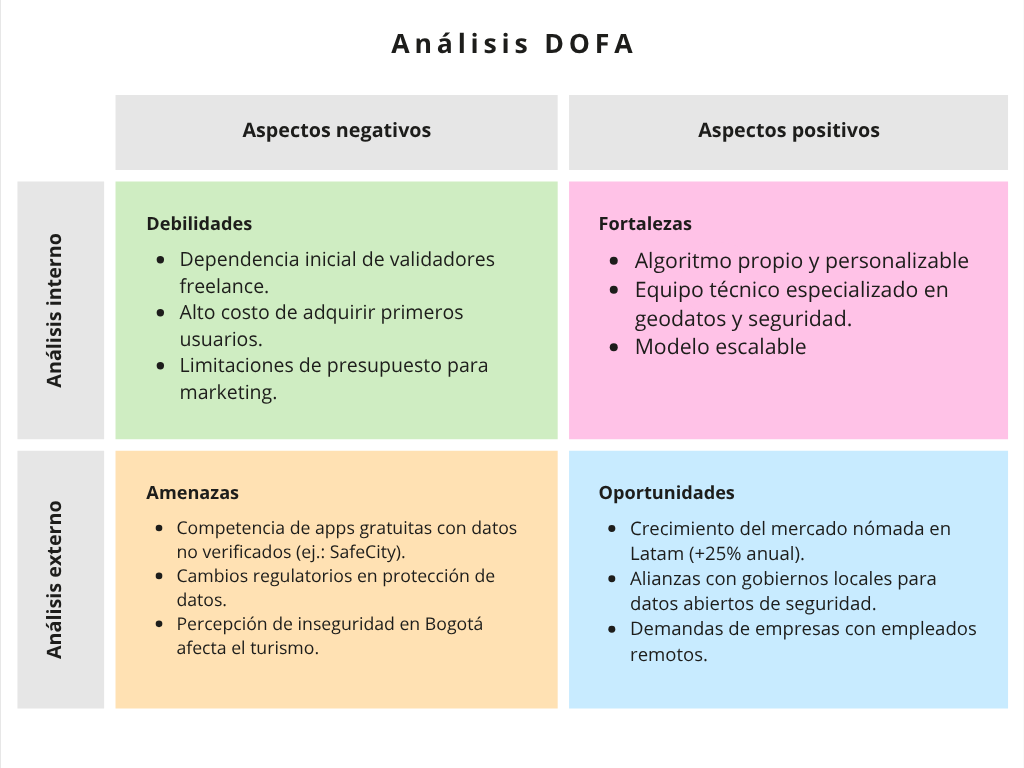
\includegraphics[width=0.6\textwidth]{Content/Images/Matriz-dofa-proyecto.png}
\footnote{Nota. \textup{Fuente : Autores.}}
\end{minipage}


